\section{Conclusions and Future Works}

The initial goal of REACH was to detect a specific grip type and perform an action as result. Although we were not able to implement it in an end-to-end manner, we believe that we have demonstrated the feasibility of such a system. It is impressive to see that the classification tree machine learning algorithm was able to accurately distinguish between 3 types of grip patterns.

\par
For future work, the following key areas were identified - 
\begin{itemize}
  \item In future prototypes, we intend to work on miniaturizing this setup and giving it the ability to wirelessly connect to phone applications (see Figure 2).
  
  \item Interface with the hardware wirelessly to collect the force sensor data. This data would then dynamically be windowed, the features extracted and the model would make a prediction, all in real-time.
  
  \item Collect a larger training dataset with the grip gestures being performed by multiple users. Explore other features that could lead to better predictions.
  
  \item Train a model that can accurately detect gestures for a large population size. This \textit{average} model could be supplemented with specific user data to increase prediction accuracy. 
  
  \item Create a user interaction scheme that dynamically responds to the grip gestures and evaluate its effectiveness.

\end{itemize}

\begin{figure}[h]
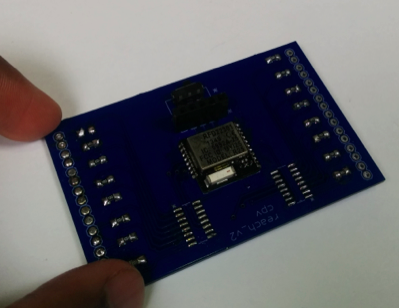
\includegraphics[width=.45\textwidth]{hardware_mini.png}
\caption{Hardware miniaturized proof of concept}
\label{fig:hardware_mini}
\end{figure}
